\documentclass{article}
\usepackage{amsmath}
\usepackage{amsfonts}
\usepackage{amsthm}
\usepackage{tikz}
\usepackage{algorithm2e}
\usepackage{fancyhdr}
\usepackage{extramarks}
\usepackage{float}

%
% Homework Details
%   - Title
%   - Due date
%   - Class
%   - Section/Time
%   - Instructor
%   - Author
%

\newcommand{\hmwkTitle}{Midterm Exam}
\newcommand{\hmwkDueDate}{April 6, 2020}
\newcommand{\hmwkClass}{MECH7710: Optimal Estimation and Control}
\newcommand{\hmwkClassInstructor}{Dr. Martin}
\newcommand{\hmwkAuthorName}{\textbf{Matthew Boler}}

%
% Homework Problem Environment
%
% This environment takes an optional argument. When given, it will adjust the
% problem counter. This is useful for when the problems given for your
% assignment aren't sequential. See the last 3 problems of this template for an
% example.
%

\setcounter{secnumdepth}{0}
\newcounter{partCounter}
\newcounter{homeworkProblemCounter}
\setcounter{homeworkProblemCounter}{1}
\nobreak\extramarks{Problem \arabic{homeworkProblemCounter}}{}\nobreak{}

\newcommand{\enterProblemHeader}[1]{
    \nobreak\extramarks{}{Problem \arabic{#1} continued on next page\ldots}\nobreak{}
    \nobreak\extramarks{Problem \arabic{#1} (continued)}{Problem \arabic{#1} continued on next page\ldots}\nobreak{}
}

\newcommand{\exitProblemHeader}[1]{
    \nobreak\extramarks{Problem \arabic{#1} (continued)}{Problem \arabic{#1} continued on next page\ldots}\nobreak{}
    \stepcounter{#1}
    \nobreak\extramarks{Problem \arabic{#1}}{}\nobreak{}
}

\newenvironment{homeworkProblem}[1][-1]{
    \ifnum#1>0
        \setcounter{homeworkProblemCounter}{#1}
    \fi
    \section{Problem \arabic{homeworkProblemCounter}}
    \setcounter{partCounter}{1}
    \enterProblemHeader{homeworkProblemCounter}
}{
    \exitProblemHeader{homeworkProblemCounter}
}

\setcounter{MaxMatrixCols}{20} % allow larger matrices

%
% Matlab code envs 
%

\usepackage{fancyvrb}
\fvset{formatcom=\color{blue},fontseries=c,fontfamily=courier,xleftmargin=4mm,commentchar=!}
\DefineVerbatimEnvironment{Code}{Verbatim}{formatcom=\color{blue},fontseries=c,fontfamily=courier,fontsize=\footnotesize,xleftmargin=4mm,commentchar=!}
\DefineVerbatimEnvironment{CodeSmall}{Verbatim}{formatcom=\color{blue},fontseries=c,fontfamily=courier,fontsize=\scriptsize,xleftmargin=1mm,commentchar=!}
\DefineVerbatimEnvironment{CodeNum}{Verbatim}{numbers=left,numbersep=4pt,formatcom=\color{blue},fontseries=c,fontfamily=courier,fontsize=\footnotesize,xleftmargin=4mm}

\newcommand{\var}[1]{{\color{blue}\Verb+#1+}}
\newcommand{\model}[1]{\index{code}{#1@\textit{#1}}\ifthenelse{\boolean{draft}}{{\color{green}\Verb+#1+}}{\Verb+#1+}}
\newcommand{\block}[1]{\ifthenelse{\boolean{draft}}{{\color{green}\Verb+#1+}}{\textsf{#1}}}
\newcommand{\func}[2][ZZZZ]{\ifthenelse{\equal{#1}{ZZZZ}}{\index{code}{#2}}{\index{code}{#1}}\ifthenelse{\boolean{draft}}{{\color{green}\Verb+#2+}}{\Verb+#2+}}
\newcommand{\methodb}[2]{\index{code}{#1@\textbf{#1}!.#2}\ifthenelse{\boolean{draft}}{{\color{magenta}\Verb+#1.#2+}}{\Verb+#1.#2+}}
\newcommand{\method}[2]{\index{code}{#1@\textbf{#1}!.#2}\ifthenelse{\boolean{draft}}{{\color{magenta}\Verb+#2+}}{\Verb+#2+}}
\newcommand{\class}[1]{\index{code}{#1@\textbf{#1}}\ifthenelse{\boolean{draft}}{{\color{cyan}\Verb+#1+}}{\Verb+#1+}}
\newcommand{\property}[1]{\index{property}{#1}\ifthenelse{\boolean{draft}}{{\color{cyan}\Verb+#1+}}{\Verb+#1+}}

\newcommand{\MATLAB}{MATLAB\textsuperscript{\textregistered}}

%
% Basic Document Settings
%

\topmargin=-0.45in
\evensidemargin=0in
\oddsidemargin=0in
\textwidth=6.5in
\textheight=9.0in
\headsep=0.25in

\linespread{1.1}
\pagestyle{fancy}
\lhead{\hmwkAuthorName}
\chead{\hmwkClass: \hmwkTitle}
\rhead{\firstxmark}
\lfoot{\lastxmark}
\cfoot{\thepage}

\title{
    \vspace{2in}
    \textmd{\textbf{\hmwkClass:\ \hmwkTitle}}\\
    \normalsize\vspace{0.1in}\small{Due\ on\ \hmwkDueDate}\\
    \vspace{3in}
}

\author{\hmwkAuthorName}
\date{}


\begin{document}

\maketitle
\pagebreak


\begin{homeworkProblem}
    Assume that $t$ observations of a random variable are given:
    \begin{align*}
        \widetilde{y}_k &= y_k \forall k = 1, ..., t
    \end{align*}
    Find a recursive formula for calculating the mean at time $t$.

    \textbf{Solution}

    Working through a series of examples,
    \begin{align*}
        \overline{y}_1 &= y_1 \\
        \overline{y}_2 &= \frac{1}{2}(\overline{y}_1 + y_2) \\
        \overline{y}_3 &= \frac{1}{3}(2\overline{y}_2 + y_3)
    \end{align*}
    the formula $\overline{y}_t = \frac{1}{t}[(t-1)\overline{y}_{t-1} + y_t]$ becomes apparent.

\end{homeworkProblem}

\newpage
\begin{homeworkProblem}
    Consider the continuous system blow
    \begin{enumerate}
        \item[a] Calculate the expected steady state Kalman filter estimation error variance
        \item[b] Calculate the steady state Kalman gaussian
        \item[c] Calculate the open loop and closed loop estimator eigenvalues
        \item[d] Plot the location of all possible closed loop eigenvalues. What do you notice about the minimum Kalman gain and the slowest closed loop estimator the Kalman filter will use?   
    \end{enumerate}

    \begin{align*}
        \dot{x} &= x + w \\
        y &= x + v \\
        E[w] &= 0 \\
        E[v] &= 0 \\
        E[ww^T] &= Q \\
        E[vv^t] &= R
    \end{align*}

    \textbf{Solution}
    Rewriting our system in a convenient form
    \begin{align*}
        \dot{x} &= Fx + Lw \\
        y &= Hx + v
    \end{align*}

    The differential equation describing the error variance is the following Riccati equation
    \begin{align*}
        \dot{P} &= FP + PF^T + LQL^T - PH^TR^{-1}HP
    \end{align*}
    as these are scalars, we simplify
    \begin{align*}
        \dot{P} &= 2FP + L^2Q - P^2H^2R^{-1} \\
        &= 2P + Q - P^2R^{-1}
    \end{align*}
    $P_{ss}$ occurs when $\dot{P} = 0$.
    Solving, we find
    \begin{align*}
        0 &= P_{ss}^2 - 2RP_{ss} - QR \\
        P_{ss} &= R \pm \sqrt{R(Q+R)} 
    \end{align*}
    Because $P$ must be positive, our steady-state error covariance $P_{ss} = R + \sqrt{R(Q+R)}$.

    The steady-state Kalman gain is given by
    \begin{align*}
        K_{ss} &= P_{ss} H^T R^{-1} \\
        &= (R + \sqrt{RQ + R^2}) R^{-1}  \\
        &= (2R + \sqrt{RQ}) R^{-1} \\
        &= 2 + \sqrt{\frac{Q}{R}}
    \end{align*}

    Our open-loop estimator eigenvalues are given by the eigenvalue of $F$, which is just $1$.

    Out close-loop estimator eigenvalues are given by the eigenvalue of $F - KH$.
    In this scalar case, the eigenvalue is equal to the value of $F - KH$.
    \begin{figure}[H]
        \centering
        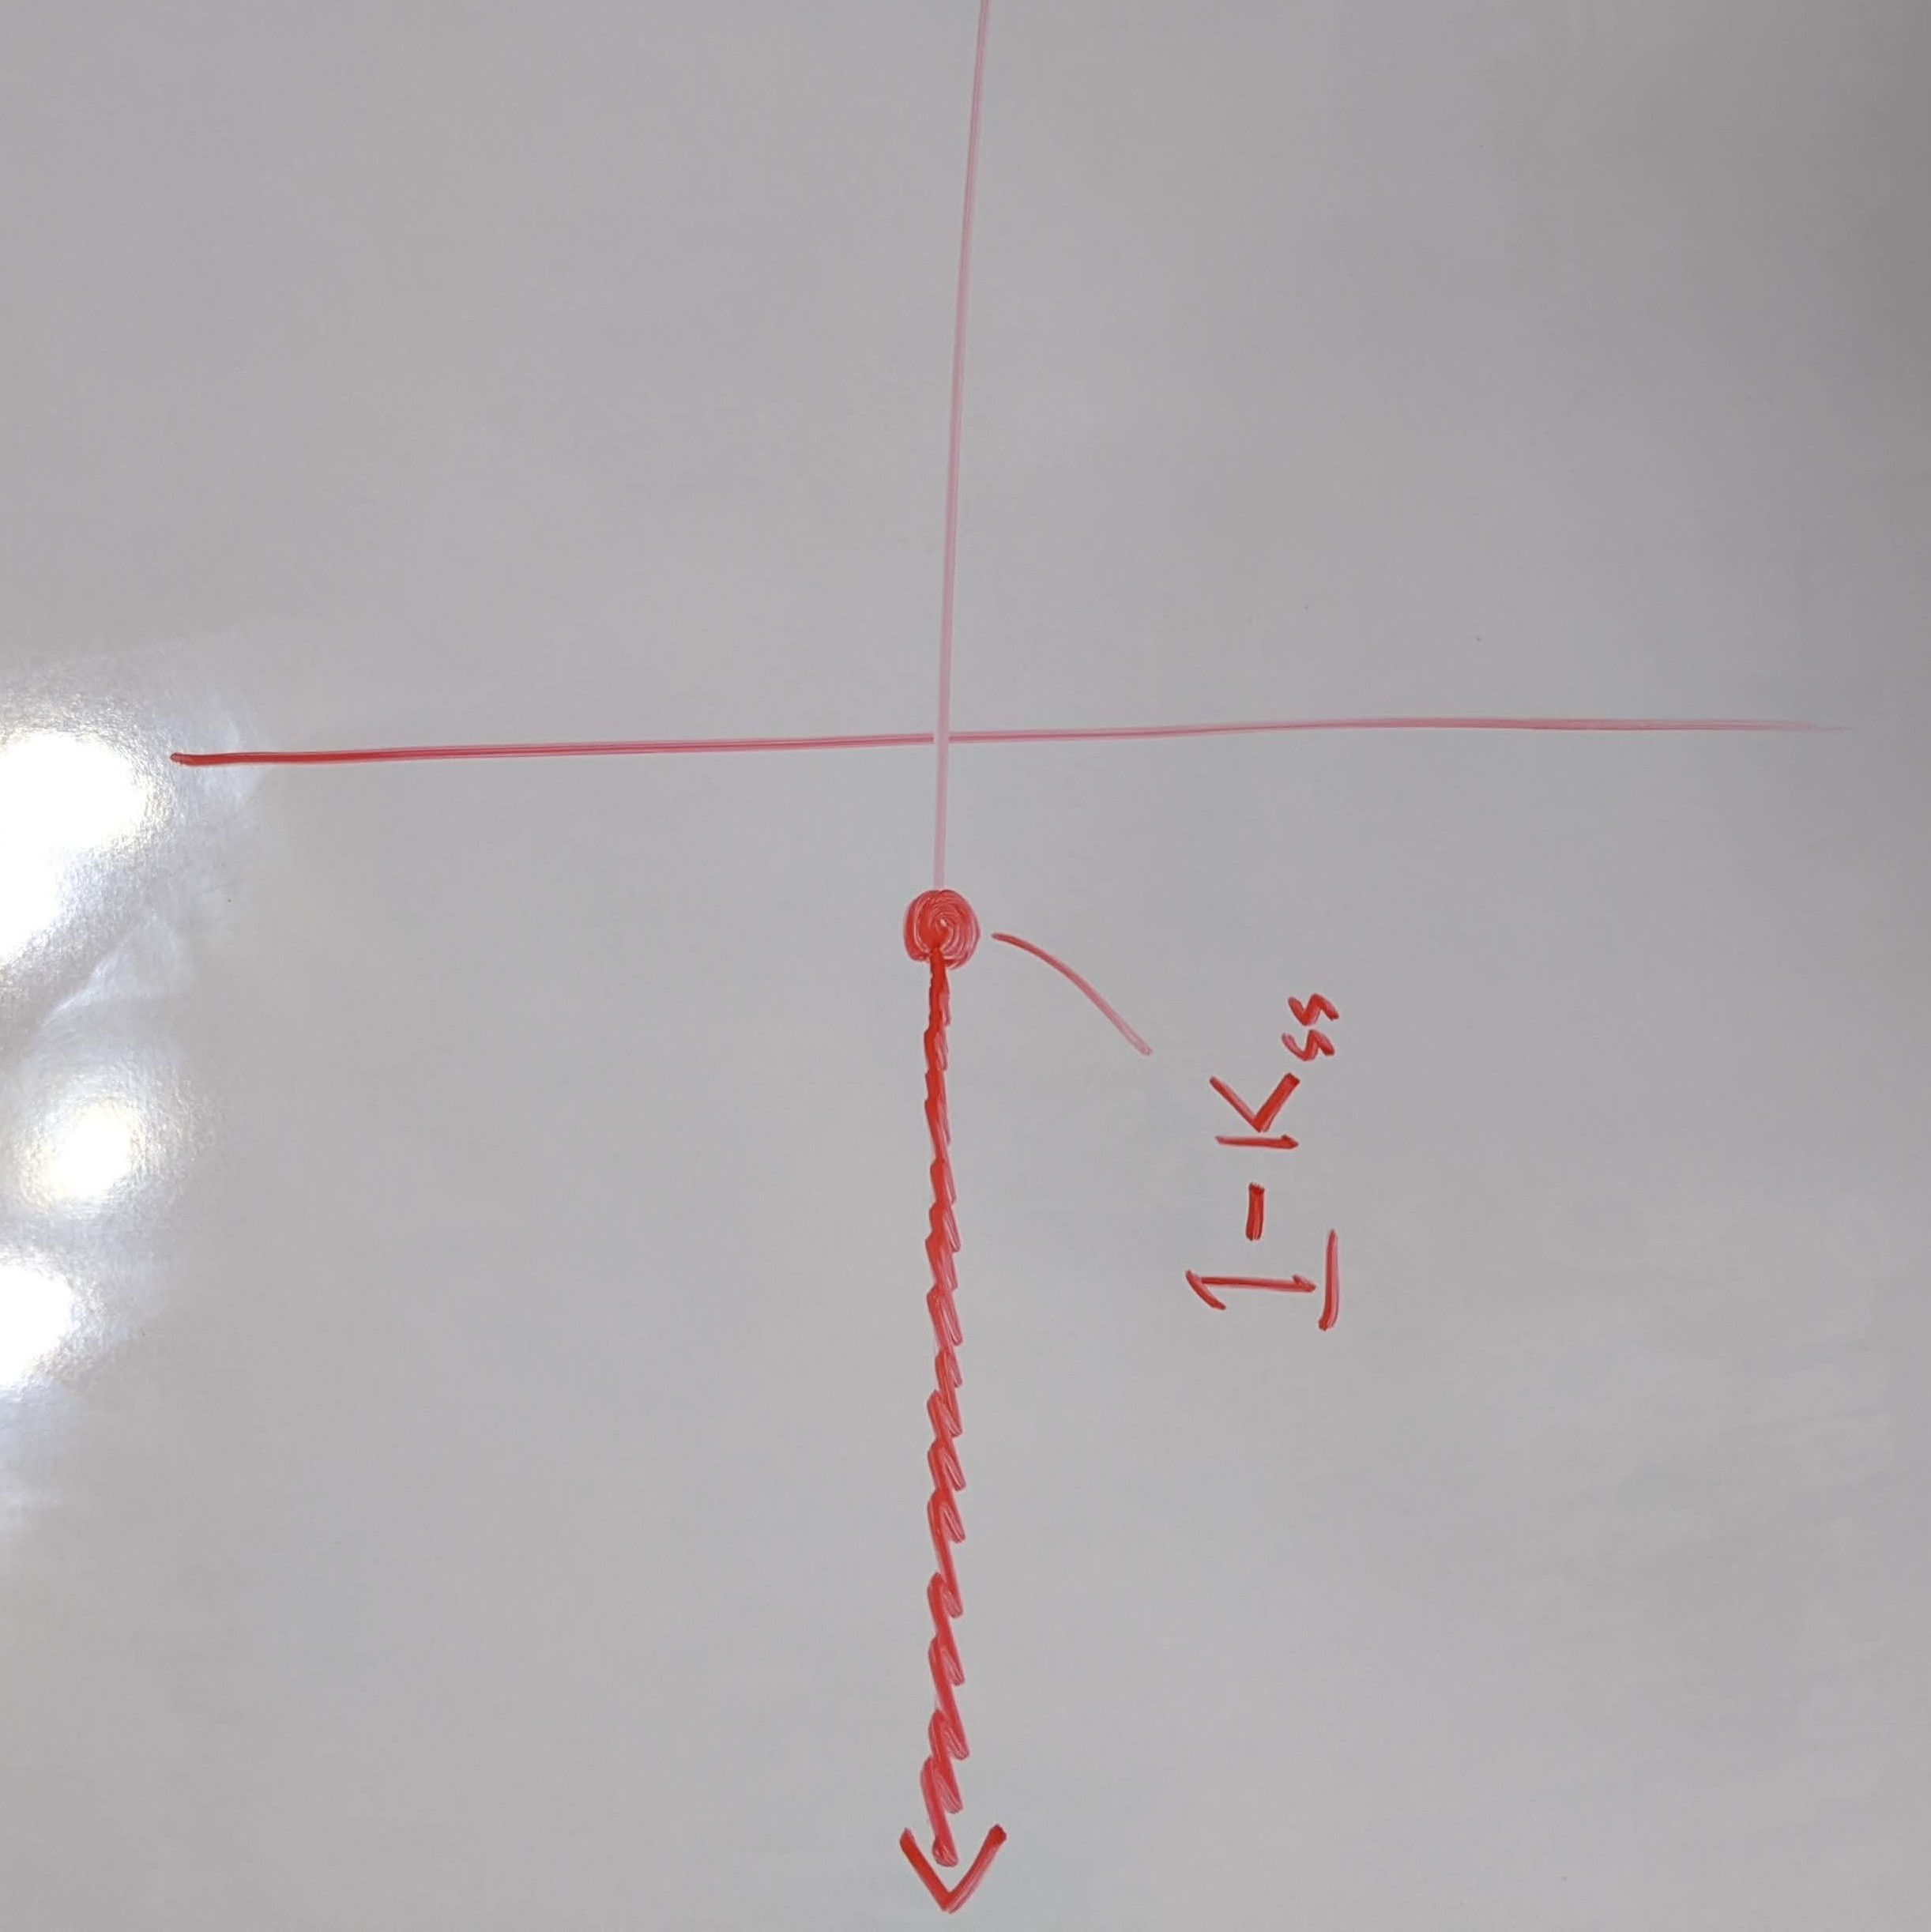
\includegraphics[width = 8cm, angle=270]{P2.jpg}
        \caption{Possible closed-loop eigenvalues}
        \label{}
    \end{figure}

    Because the steady-state error covariance represents the minimum of a quadratic function, it is the lower bound of the Kalman gain and all possible eigenvalues lay in $\lambda \in ( - \infty, 1 - K_{ss}]$.
    Clearly, the eigenvalue corresponding to the steady-state Kalman gain is the slowest, while eigenvalues corresponding to higher covariances are faster.

    
    
\end{homeworkProblem}

\newpage
\begin{homeworkProblem}
    Given the measurements shown in the table:
    \begin{enumerate}
        \item[a] Use least squares to estimate the slope and y-intercept of a line assuming the x values are the inputs and the y values are measurements that are corrupted by zero-mean Gaussian noise with a standard deviation of 0.2
        \item[b] What is the expected error of the estimate?
        \item[c] Use weighted least squares to calculate the estimates assuming the last measurement is twice as bad (1 $\sigma$) as the first two measurements.  
    \end{enumerate}

    \begin{table}[H]
        \centering
        \begin{tabular}{c|c|c}
            k & x & y \\
            1 & 0 & 3 \\
            2 & 1 & 2 \\
            3 & 2 & 0
        \end{tabular}
    \end{table}

    \textbf{Solution}

    Since our system is $ y = ax + b$, our $H$ matrix is:
    $\begin{bmatrix}
        0 & 1 \\
        1 & 1 \\
        2 & 1
    \end{bmatrix}$, our $Y$ matrix is 
    $\begin{bmatrix}
        3 \\
        2 \\
        0
    \end{bmatrix}$, and our $X$ matrix is 
    $\begin{bmatrix}
        a \\
        b
    \end{bmatrix}$.

    Our estimate of $X$ is then $(H^TH)^{-1}H^TY$, which gives us 
    \begin{align*}
        a &= -1.5 \\
        b &= 3.1667
    \end{align*}

    The expected error of this estimate is 0, as the linear least squares estimator is unbiased.

    If we assume that the last measurement is twice as bad as the first two, we construct the weighting matrix $W = \begin{bmatrix}
        \frac{1}{0.2} & 0 & 0 \\
        0 & \frac{1}{0.2} & 0 \\
        0 & 0 & \frac{1}{0.4}
    \end{bmatrix}$, and our new estimate of $X$ is $ (H^T W H)^{-1} H^T W Y $, which gives us
    \begin{align*}
        a &= -1.4286 \\
        b &= 3.1429
    \end{align*}



\end{homeworkProblem}

\newpage
\begin{homeworkProblem}
    A random number generator generates integers from 1 to 9 (inclusive). All outcomes are equally likely, and each integer is generated independently of any previous integer. Let $\Sigma$ denote the sum of two consecutively generated integers.

    \begin{enumerate}
        \item[a] Given $N_1 > 8$, what is the probability that $\Sigma$ is odd?
        \item[b] Given $\Sigma > 10$, what is the probability that at least one of the integers is greater than 7?
        \item[c] Using Bayes' rule, find the conditional probability that $\Sigma = 7$ given $\Sigma$ is odd.  
    \end{enumerate}

    \textbf{Solution}

    Our sample space is represented by the table below.
    \begin{table}[H]
        \centering
        \label{tb1}
        \begin{tabular}{ccccccccc}
            2 & 3 & 4 & 5 & 6 & 7 & 8 & 9 & 10 \\
            3 & 4 & 5 & 6 & 7 & 8 & 9 & 10 & 11 \\
            4 & 5 & 6 & 7 & 8 & 9 & 10 & 11 & 12 \\
            5 & 6 & 7 & 8 & 9 & 10 & 11 & 12 & 13 \\
            6 & 7 & 8 & 9 & 10 & 11 & 12 & 13 & 14 \\
            7 & 8 & 9 & 10 & 11 & 12 & 13 & 14 & 15 \\
            8 & 9 & 10 & 11 & 12 & 13 & 14 & 15 & 16 \\
            9 & 10 & 11 & 12 & 13 & 14 & 15 & 16 & 17 \\
            10 & 11 & 12 & 13 & 14 & 15 & 16 & 17 & 18
        \end{tabular}
    \end{table}

    $N_1 > 8$ means $N_1 = 9$. If $N_2 \in {2, 4, 6, 8}$ then $\Sigma$ is odd; otherwise if $N_2 \in {1, 3, 5, 7, 9}$ then $\Sigma$ is even. Thus, $P(\Sigma \: odd \vert N_1 > 8) = \frac{4}{9}$.
    \medskip

    $\Sigma > 10$ removes the upper left corner and diagonal of the sample space, reducing the number of events by 45. Of the remaining 36, 11 involve generating a 7. Thus, $P(N_1 = 7 \: or \: N_2 = 7 \vert \Sigma > 10) = \frac{11}{36}$. 
    \medskip

    Using Bayes' rule we wish to find $P(\Sigma = 7 \vert \Sigma \: odd)$.
    We need:
    \begin{itemize}
        \item $P(\Sigma \: odd) = \frac{40}{81}$
        \item $P(\Sigma \: odd \vert \Sigma = 7) = 1$
        \item $P(\Sigma = 7) = \frac{6}{81}$
    \end{itemize}
    From these we find $P(\Sigma = 7 \vert \Sigma \: odd) = P(\Sigma \: odd \vert \Sigma = 7) \frac{P(\Sigma = 7)}{P(\Sigma \: odd)} = 0.15$.
    

\end{homeworkProblem}

\newpage
\begin{homeworkProblem}
    Consider the linearized pendulum driven by a motor torque with a force disturbance. The system is sampled at 100Hz. The pendulum has an optical encoder with 360 counts/revolution to measure angular position. The motor has a tachometer that measures angular velocity with an accuracy of 0.2 deg/s (1 $\sigma$). However, the tachometer measurement has a bias that should be modeled as a markov process with a time constant of 10 seconds and a unit white noise input.

    \begin{align*}
        J\ddot{\theta} + b \dot{\theta} + mgl\theta &= \tau_m - F_dl \:\: where \:\: E[F_d] = \mu_d \:\: and \:\: E[F_dF_d^T] = \sigma_d^2
    \end{align*}

    \begin{enumerate}
        \item[a] Find $A, B_u, B_w, C, D, Q, R$ 
        \item[b] Find the first order approximation of $A_d$
        \item[c] Calculate $Q_d$  
    \end{enumerate}

    \textbf{Solution}
    We define
    \begin{itemize}
        \item $t_c = 10s$
        \item $\beta$ is the tachometer bias
        \item $dt = \frac{1}{100}s$
    \end{itemize}

    An additional note: no noise parameters are given for the encoder, so we assume perfect measurements (unrealistic but simple). 
    We could assume that the true angle is uniformly distributed between clicks, in which case the variance would be $\frac{1}{12}(\frac{1}{360})^2$.

    We want our system in the form
    \begin{align*}
        \dot{x} = Ax + B_u u + B_w \omega \\
        y = Cx + Du + \nu_s
    \end{align*}

    Our state space model is as follows
    \begin{align*}
        \frac{d}{dt}
        \begin{bmatrix}
            \dot{\theta} \\
            \theta \\
            \beta \\
            \mu_d
        \end{bmatrix} &= \begin{bmatrix}
            -\frac{b}{J} & -\frac{mgl}{J} & 0 & -\frac{l}{J} \\
            1 & 0 & 0 & 0 \\
            -\frac{1}{t_c} & 0 & 0 & 0 \\
            0 & 0 & 0 & 0
        \end{bmatrix} \begin{bmatrix}
            \dot{\theta} \\
            \theta \\
            \beta \\
            \mu_d
        \end{bmatrix} + \begin{bmatrix}
            \frac{1}{J} \\
            0 \\
            0 \\
            0
        \end{bmatrix} \tau_m + \begin{bmatrix}
            -\frac{l}{J} & 0 \\
            0 & 0 \\
            0 & 1 \\
            0 & 0 
        \end{bmatrix} \begin{bmatrix}
            \omega_{\tau} \\
            \omega_{\beta}
        \end{bmatrix} \\
        \begin{bmatrix}
            \dot{\theta} \\
            \theta
        \end{bmatrix} &= \begin{bmatrix}
            1 & 0 & 1 & 0 \\
            0 & 1 & 0 & 0
        \end{bmatrix} \begin{bmatrix}
            \dot{\theta} \\
            \theta \\
            \beta \\
            \mu_d
        \end{bmatrix} + \begin{bmatrix}
            0
        \end{bmatrix} \tau_m + 
        \begin{bmatrix}
            1 \\ 
            0
        \end{bmatrix} \nu_s \\
        Q &= \begin{bmatrix}
            \sigma_d^2 & 0 \\
            0 & 1
        \end{bmatrix} \\
        R &= \begin{bmatrix}
            0.04deg/s & 0 \\
            0 & 0
        \end{bmatrix}
    \end{align*}

    The first-order approximation of $A_d$ is 
    \begin{align*}
        A_d \approx I + Adt
    \end{align*}

    Our $Q_d$ is 
    \begin{align*}
        Q_d = B_w  Q  B_w^T dt
    \end{align*}

\end{homeworkProblem}



\end{document}